%
\begin{frame}
\frametitle{}
\begin{center}
  \textbf{\Large The multi-objective knapsack problem}
\end{center}
\end{frame}

% MO problems
\begin{frame}
\frametitle{Multi-objective optimization problems}
\begin{block}{Definition}
  A general multi-objective optimization problem can be described as a vector
  function $f$ that maps a decision variable (solution) to a tuple
  of $\np$ objectives. \pause
\begin{align*}
  \text{max} ~ \sol{y} &= f(\sol{x}) =
    \big(f_1(\sol{x})
    ,f_2(\sol{x})
    ,\ldots
    ,f_{\np}(\sol{x})\big) \\
  \text{subject to} ~ \sol{x} & \in X
\end{align*}
\end{block}
\pause
\qquad $\sol{x}$ is the \emph{decision variable}; \pause \\
\qquad $X$ denotes the set of feasible solutions; \pause \\
\qquad $\sol{y}$ is the \emph{objective vector}, each one has to be maximized.
\end{frame}

% Dominance
\begin{frame}
\frametitle{Multi-objective optimization problems}
\begin{block}{Dominance}
  Consider two decision vectors $\sol{a}, \sol{b} \in X$.
  \pause
  Vector $\sol{a}$ \emph{dominates} $\sol{b}$ \pause
   if, and only if \pause
   $\sol{a}$ is at least as good as $\sol{b}$
  in all objectives \pause
  and better than $\sol{b}$ in at least one objective. \pause
\begin{displaymath}
    \dom{a}{b} = \left\{
      \begin{array}{l}
          \forall i \in \{1, 2, \ldots, \np\}: f_i(\sol{a}) \geq f_i(\sol{b}) ~\text{and}\\
          \exists j \in \{1, 2, \ldots, \np\}: f_j(\sol{a}) > f_j(\sol{b})
  \end{array} \right.
\end{displaymath}
\end{block} \pause
\begin{block}{Efficiency}
A feasible solution $\sol{x} \in X$ is called \emph{efficient} %or \emph{non-dominated}
if it is not dominated by any other feasible solution. \pause
\begin{displaymath}
    efficient(\sol{x}) = \nexists \sol{a} \in X: \dom{a}{x}
\end{displaymath} \pause
\end{block}
\begin{block}{Pareto set}
The set of all efficient solutions.\pause
\begin{displaymath}
    Pareto(X) = \{ \sol{x} \in X: efficient(\sol{x}) \}
\end{displaymath}
\end{block}
\end{frame}

\begin{frame}
\frametitle{Multi-objective optimization problems}
\begin{figure}
  \centering
  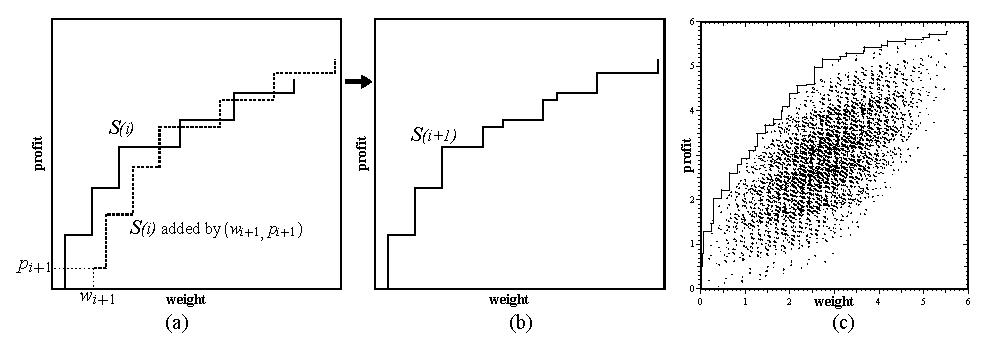
\includegraphics{img/pareto}
  \caption{Example of a Pareto set for a bi-objective problem.}
\end{figure}
\end{frame}

% Problem Definition
\begin{frame}
\frametitle{The multi-objective knapsack problem}
\begin{block}{Problem Definition}
A problem instance with $n$ items and $m$ objectives:
\begin{align*}
  \text{max   } & f(\sol{x}) =
    \big(f_1(\sol{x}) ,f_2(\sol{x}) ,\ldots ,f_{\np}(\sol{x})\big) \\
  \text{subject to   } & w(\sol{x}) \leq W \\
  & \sol{x} \subseteq \setIN\\
\end{align*}
\pause
\vspace{-35pt}
\begin{align*}
  \text{where} \phantom{mmmmm} \\
  f_j(\sol{x}) &= \sum_{i \in \sol{x}} p^j_i \quad j = 1, \ldots, m\\
  w(\sol{x}) &= \sum_{i \in \sol{x}} w_i
\end{align*}
\end{block} \pause
A \nphard{} problem for which the Pareto optimal set
tends to grow exponentially with the number of objectives.
\end{frame}

% Knapsack dominance
\begin{frame}
\frametitle{The multi-objective knapsack problem}
\begin{block}{Knapsack dominance}
Consider two solutions $\sol{x}, \sol{y}$ for a MOKP.
\medskip \\
We say $\sol{x}$ \emph{knapsack-dominates} $\sol{y}$, denoted as $\domk{x}{y}$,
if $\sol{x}$ dominates $\sol{y}$ and does not weight more than $\sol{y}$.
\pause
Formally:
\begin{equation*}
  \label{eq:kdom}
  \domk{x}{y} = \left\{
    \begin{array}{l}
      \dom{x}{y} \quad \text{and} \\
      w(\sol{x}) \leq w(\sol{y})
    \end{array}
  \right.
\end{equation*}
\end{block}
\pause
\begin{figure}
  \centering
  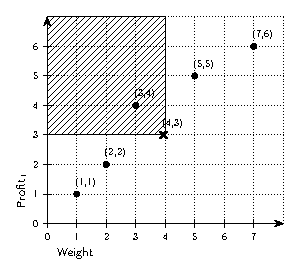
\includegraphics[scale=0.8]{img/kdt/dom}
  \caption{A knapsack-dominated solution.}
\end{figure}
\end{frame}
